\documentclass[journal]{IEEEtran}

\usepackage[pdftex]{graphicx}
\graphicspath{{img/}}
\usepackage{cite}
\usepackage{amsmath}
\usepackage{mathtools}
\usepackage{booktabs,siunitx}
\usepackage{threeparttable}
%\usepackage{subcaption}
\usepackage{multirow}
\usepackage[caption=false,font=footnotesize,labelfont=sf,textfont=sf]{subfig}

\usepackage{endfloat}

% TODO: remove
	\usepackage{xcolor}
	\newcommand\TODO[1]{\textcolor{red}{TODO: #1}}
	\newcommand\FIXME[1]{\textcolor{blue}{FIXME: #1}}

\begin{document}
\title{Title of the Paper}


\author{Michael~Mueller,
        Jan~Riedo,
        Michael~Rebsamen% <-this % stops a space
\thanks{Biomedical Engineering, University of Bern}% <-this % stops a space
\thanks{Authors e-Mail: michael.mueller4@students.unibe.ch, jan.riedo@students.unibe.ch, michael.rebsamen@students.unibe.ch}}% <-this % stops a space
\markboth{Biomedical Engineering, Medical Image Analysis Lab, \today}%
{Title of the Paper}
\maketitle

\begin{abstract}
Machine learning (ML), white matter (WM), grey matter (GM), cerebrospinal fluid (CF), background (BG)
\end{abstract}
\begin{IEEEkeywords}
MRI, Segmentation, Machine Learning, DF, kNN, SVM
\end{IEEEkeywords}


\section{Introduction}
Segmentation of brain tissues from magnetic resonance images (MRI) has many clinical applications. Clinicians gain useful information from a separation of tissue into its three main anatomical types: white matter, grey matter, and ventricles. However, manual segmentation of MRI is a labour-intensive task requiring expert skills. Fully automatic approaches for brain tissue segmentation are therefore a topic of active research. A good algorithm classifies the tissue types with high accuracy across a variety of images from different patients. Such a classification is a typical task for machine learning. These algorithms tend to perform well given enough training data during the learning phase. The availability of ground-truth data in sufficient quantity and quality for supervised learning is a particular challenge when working with medical images due to privacy concerns and the costs for manual segmentation. Optimization of the learning phase with a limited number of training data is therefore required.

\FIXME{kNN is a popular classification method for MR data and has successfully been applied in MR brain segmentation\cite{Anbeek2004,Cocosco2003,Warfield2000}}

\FIXME{Base paper on df \cite{Breiman2001}.}


\section{Methods}

\subsection{Dataset}
All experiments were conducted on a subset of 100 unrelated subjects from a dataset provided by the \textit{Human Connectome Project} \cite{van2013wu}. From each individual, a total of eight 3-tesla head MRI are available: T1 and T2-weighted image volumes not skull-stripped (but defaced for anonymization) and skull-stripped with a bias field correction, and both modalities once in native T1 space and once in MNI-atlas space \cite{mazziotta2001probabilistic}.

Ground-truth labels are automatically generated using \textit{FreeSurf}, assigning each voxel either to background, white matter, grey matter, or ventricles. The dataset was split in a training set with 70 images and a test set with 30 images.

\subsection{Pipeline}

Training and testing data are loaded sequentially, each put through the pipeline consisting of: registration, pre-processing, feature extraction and ML training/classification. For testing, two additional steps, namely post-processing and evaluation are added.

Firstly, the data is loaded and registered to an atlas with a multi-modal rigid transformation using a regular step gradient descent optimizer. \FIXME{In the preprocessing module skull stripping and bias field correction are applied in order to have images of the brain only, with less influence of the MRI scanning characteristics. Furthermore, a gradient anisotropic diffusion filter and z-score normalization is applied.}

Preprocessed data is then fed into the feature extraction module, where seven features are computed. The feature matrix consists of three coordinate features, a T1 and a T2 intensity feature, and a T1 and T2 gradient feature. During feature extraction, a random mask is applied in order to randomly select a fraction of the voxels available. The mask is adjustable individually for BG, WM, GM, and CF. This is where the pathways of training and testing split up: training data is lastly fed to a certain supervised machine learning algorithm for training, whereas the testing data is classified with the previously created model. The classified testing data is then forwarded to a post-processing module where a dense conditional random field \cite{krahenbuhl2011efficient} is applied.
Finally, the classification is evaluated based on a comparison with the ground truth, where a dice coefficient is computed (see chap.~\ref{ch.eval}).


\FIXME{The medical image analysis pipeline consists of seven phases. In the pre-processing phase, an intensity normalization is performed on the images to have comparable grey scale ranges among all images in the subsequent steps. Similarly, the registration phase registers the images to an atlas space to have a common coordinate system. In the feature extraction phase, seven features are calculated for each voxel: three coordinates corresponding to the position of the voxel in the atlas space, and an intensity and a gradient on both the T1 and T2 modalities. A subset of voxels is choosen randomly to be used for training. During the learning phase, the selected algorithm is trained to classify voxels based on the given features. In the segmentation phase, the trained algorithm is used to classify all voxels in previously unseen test images. The post-processing phase aims to reduce noise by eliminating small isolated regions with a dense conditional random field \cite{krahenbuhl2011efficient}. Finally, the evaluation phase assesses the performance of the segmentation by comparing the result to ground-truth and calculating a dice coefficient for each class.}

\subsection{Training}
\TODO{Describe training of machine learning algorithms}
\TODO{\textbf{Short} intro to used algorithms?}

\subsection{Support Vector Machine (SVM)}
Classification using Support Vector Machines (SVM) tries to find a hyperplane separating the data in a high-dimensional feature space. Given the feature vector $x_i$ and the binary label $y_i$, the SVM solves the following optimization problem during training:
\begin{equation}
\begin{split}
\min_{w, b, \xi} \ & \frac{1}{2}w^Tw + C\sum_{i=1}^m \xi_i \\
\ \text{ s.t. } & y_i(w^T\phi(x_i)+b) \geq 1-\xi_i, \; i = 1, \ldots, m \\
& \xi_i \geq 0, \; i = 1, \ldots, m
\end{split}
\end{equation}
where $w$ is the normal vector and $b$ the offset of the separating hyperplane and $\phi(x_i)$ maps $x_i$ into a higher-dimensional space.

The SVM implementation is based on libSVM \cite{chang2011libsvm}. Multiclass classification is solved with a \textit{one-against-one} approach. To output probabilities, the predictions are calibrated using \textit{Platt} scaling in which multiclass problems require an additional cross-validation which is an expensive operation for large datasets.

Given the relative low number of available features, we have chosen a radial basis function (RBF) kernel. A regularization term $C$ and a model capacity $\gamma$ needs to be chosen. These hyperparameters were determined with an exhaustive search and cross-validated on a subset of the training data, yielding $C=500$ and $\gamma=0.00005$.

\subsection{Performance Evaluation}\label{ch.eval}
The Dice coefficient is a commonly used metric to compare the spatial overlap, ranging from 0 (no overlap) to 1 (perfect overlap). To evaluate the accuracy of the segmentation, a Dice coefficient is calculated between the prediction (E) and ground-truth (G) for each of the three labels. 
\begin{equation}
D = \frac{2|E \bigcap G|}{|E| + |G|} = \frac{2 TP}{2 TP + FP + FN}
\end{equation}

\subsection{Infrastructure}
\TODO{Describe UBELIX, libraries}


\section{Results}
All algorithms tested and optimized were able to yield a good result for brain segmentation. The performance measured with the dice coefficient can be found in Tab.~(\ref{tab:perf_compare}). Comparisons of computation time can be seen in Tab.~(\ref{tab:time_compare}).\\

\subsection{Ground Truth Validity}

The importance of looking at the images and not only at the numbers shall be presented based on one example MRI image, segmented with kNN. In Fig.~(\ref{f.ground_truth}) we see one slice of a brain, segmented in three different ways. On the left, we see a kNN segmentation based on non-coordinate features. The one in the middle is segmented with kNN based on all features. On the right we see the ground truth. Although the middle image shows a substantially better result in ventricle dice than the left (0.68 vs. 0.76) we can barely see an improved ventricle segmentation with bare eyes. What we see however, is a big difference on how detailed the white and grey matter are segmented, thus leading to a better overall segmentation. Another fact which shall be presented here is that the ground truth image is not a real ground truth. It is an image segmented by another algorithm. In Fig~(\ref{f.knn_a}) a better segmentation of the center part (white matter) is achieved compared to the ground truth image in Fig~(\ref{f.knn_c}) (background).

\begin{figure*}
	\centering
	\subfloat[]{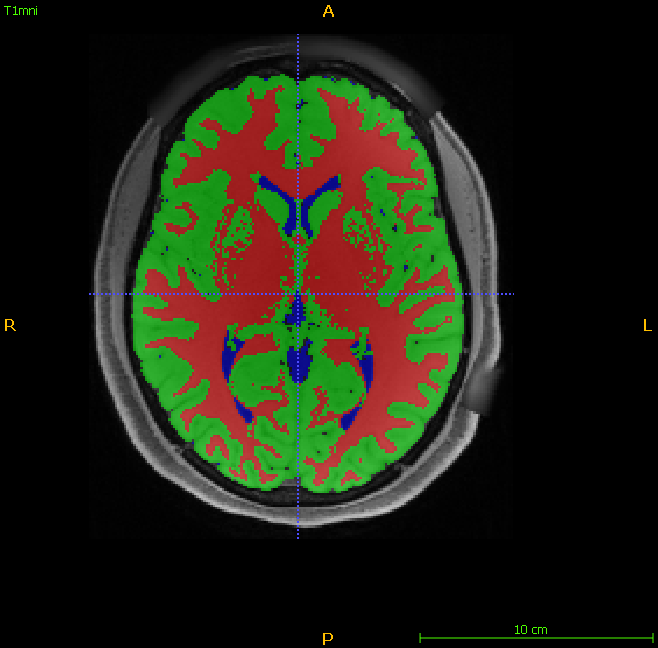
\includegraphics[width=0.3\linewidth]{images/knn_no_coord}\label{f.knn_a}}
	\hfill
	\subfloat[]{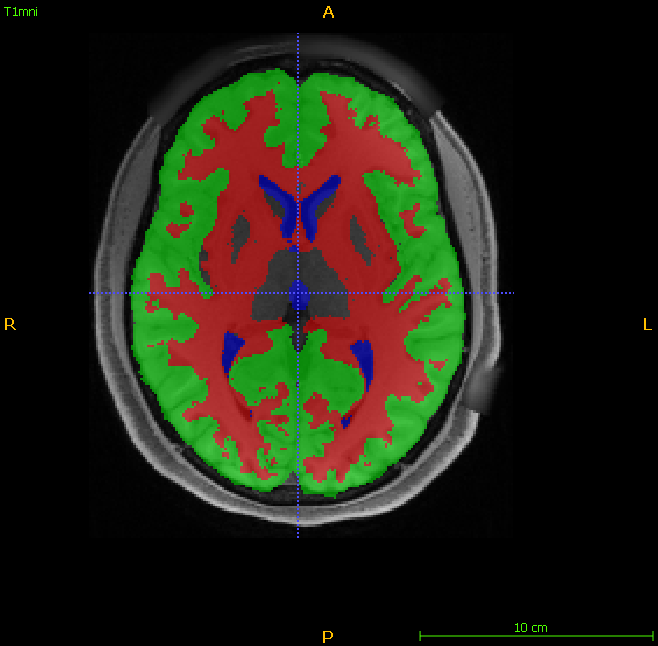
\includegraphics[width=0.3\linewidth]{images/knn_all}}
	\hfill
	\subfloat[]{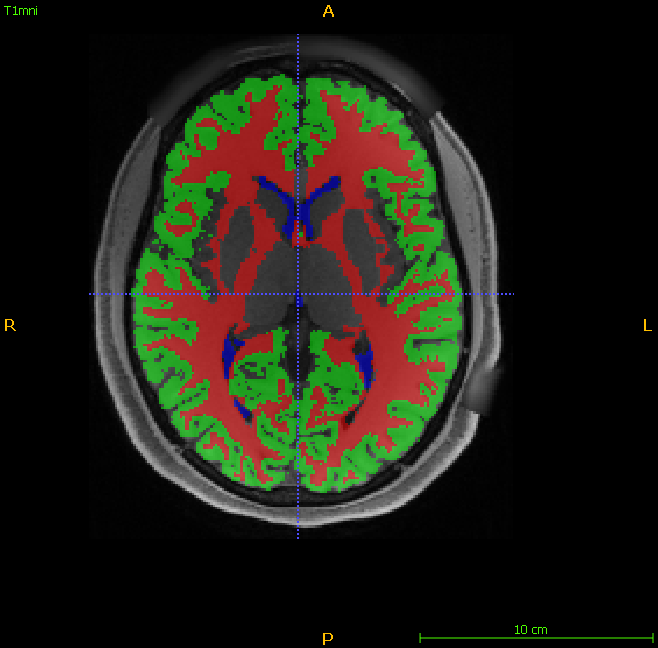
\includegraphics[width=0.3\linewidth]{images/knn_ground_truth}\label{f.knn_c}}
	\caption{(a) kNN segmented image based on non-coordinate features with dice values 0.86/0.82/0.68. (b) kNN segmented image based on all features with dice values 0.80/0.79/0.76. (c) Ground truth.}
	\label{f.ground_truth}
\end{figure*}

\subsection{Feature Inspection}

Feature selection is another key part of the machine learning process. Features are also called variable or attribute and describe the model. Irrelevant and redundant features do not contribute to the accuracy of the predictive model, at worst they decrease the accuracy. The used feature set consists of seven features, f1-f3: Coordinate features, f4: T1 intensity, f5: T1 gradient, f6: T2 intensity, f7: T2 gradient. The following Fig~(\ref{scatterplot}) shows the scatter matrix of all the features. On the diagonal are the histograms for each feature. The right upper part of the diagonal visualizes the linear correlation between each of the feature with the associated correlation coefficient. The left bottom part of the diagonal is redundant to the upper part. There is a moderate uphill relationship for the feature f4 \& f5, f5 \& f6, f5 \& f7. A strong uphill linear relationship for coefficients over 0.7, in this case for the feature f6 \& f7. This imply, that only the the first three feature, the coordinates, are independent.

\begin{figure}
	\centering
	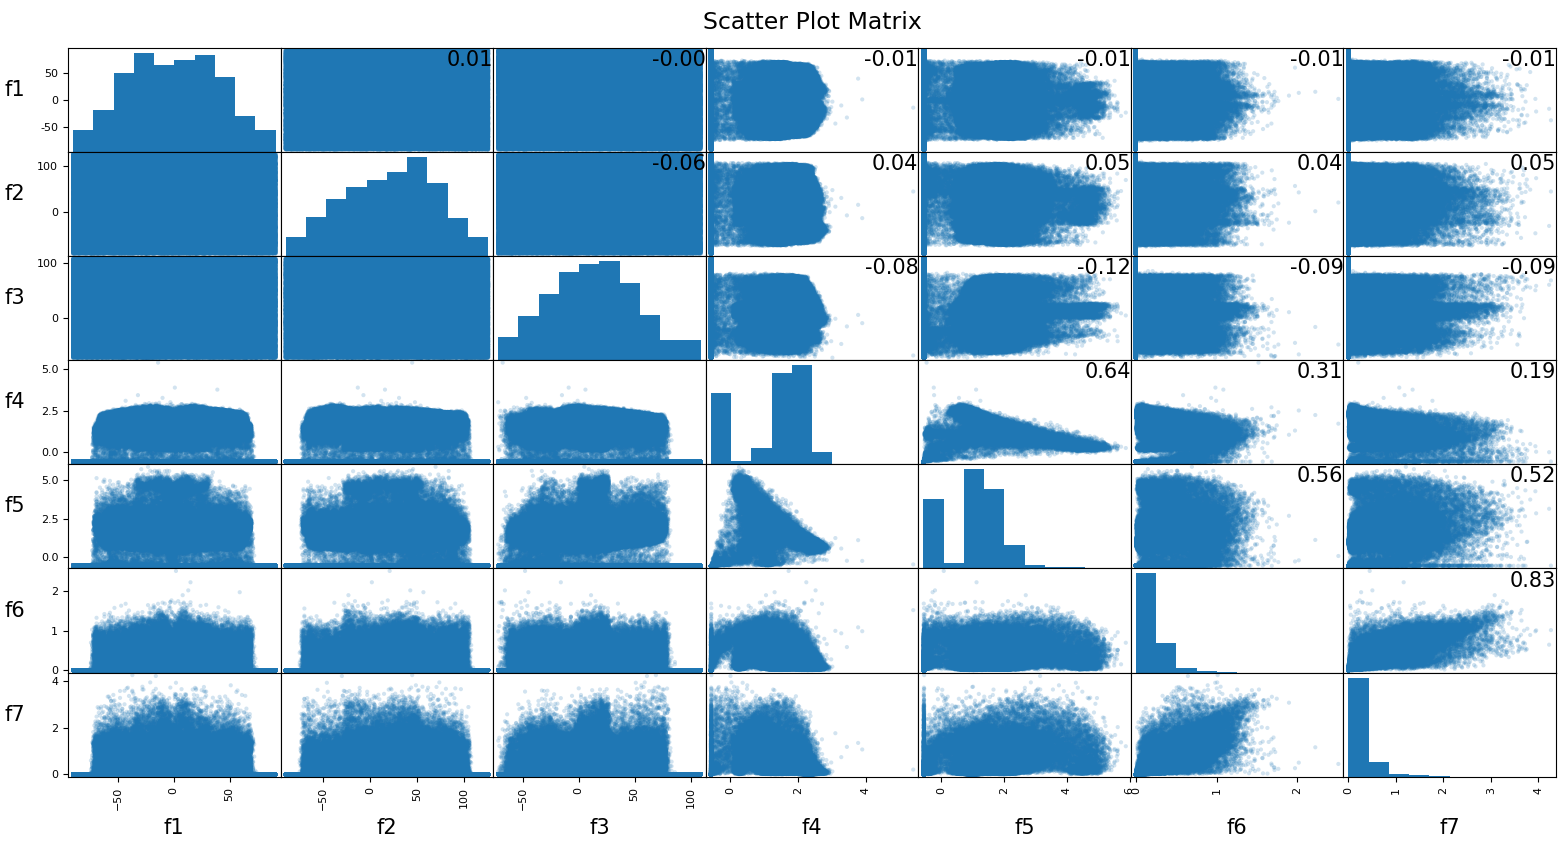
\includegraphics[width=0.48\textwidth]{images/ScatterPlotMatrix}
	\caption{Scatter plot of the features with correlation coefficient}
	\label{scatterplot}
\end{figure}


\begin{figure}
	\centering
	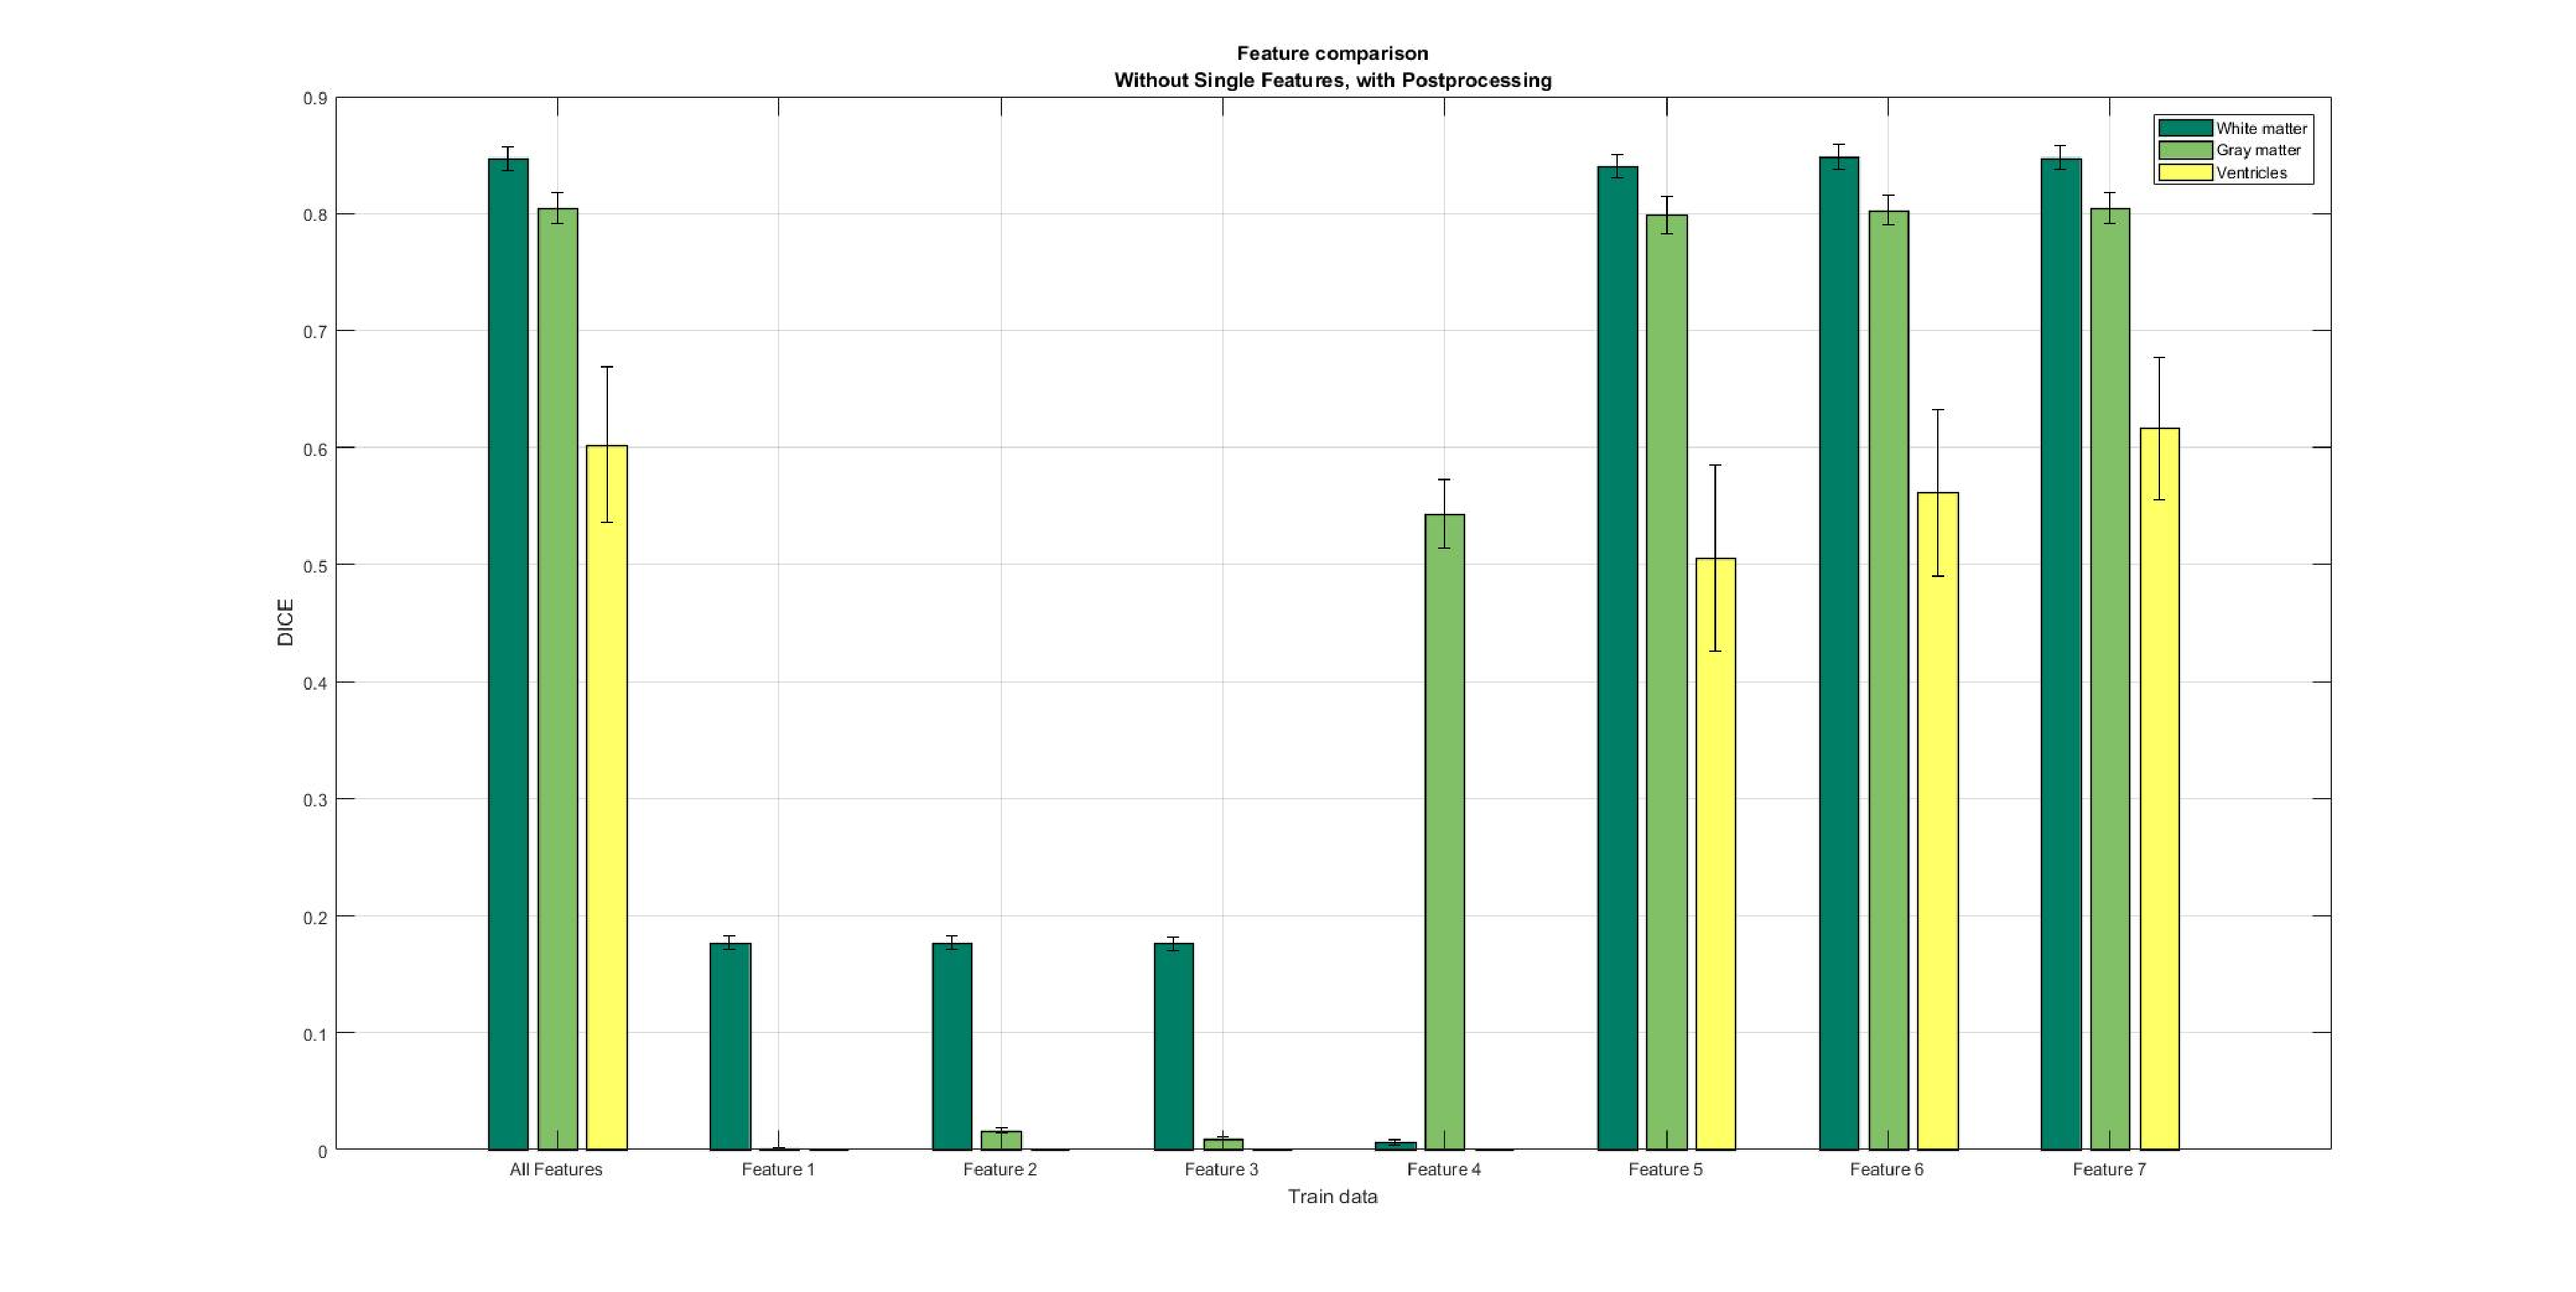
\includegraphics[width=0.48\textwidth]{images/DF_FE_WSF_PP}
	\caption{Feature evaluation with Decision Forest by removing a single feature and with preprocessing}
	\label{DF_FeatEval_WSF_PP}
\end{figure}


\begin{figure}
	\centering
	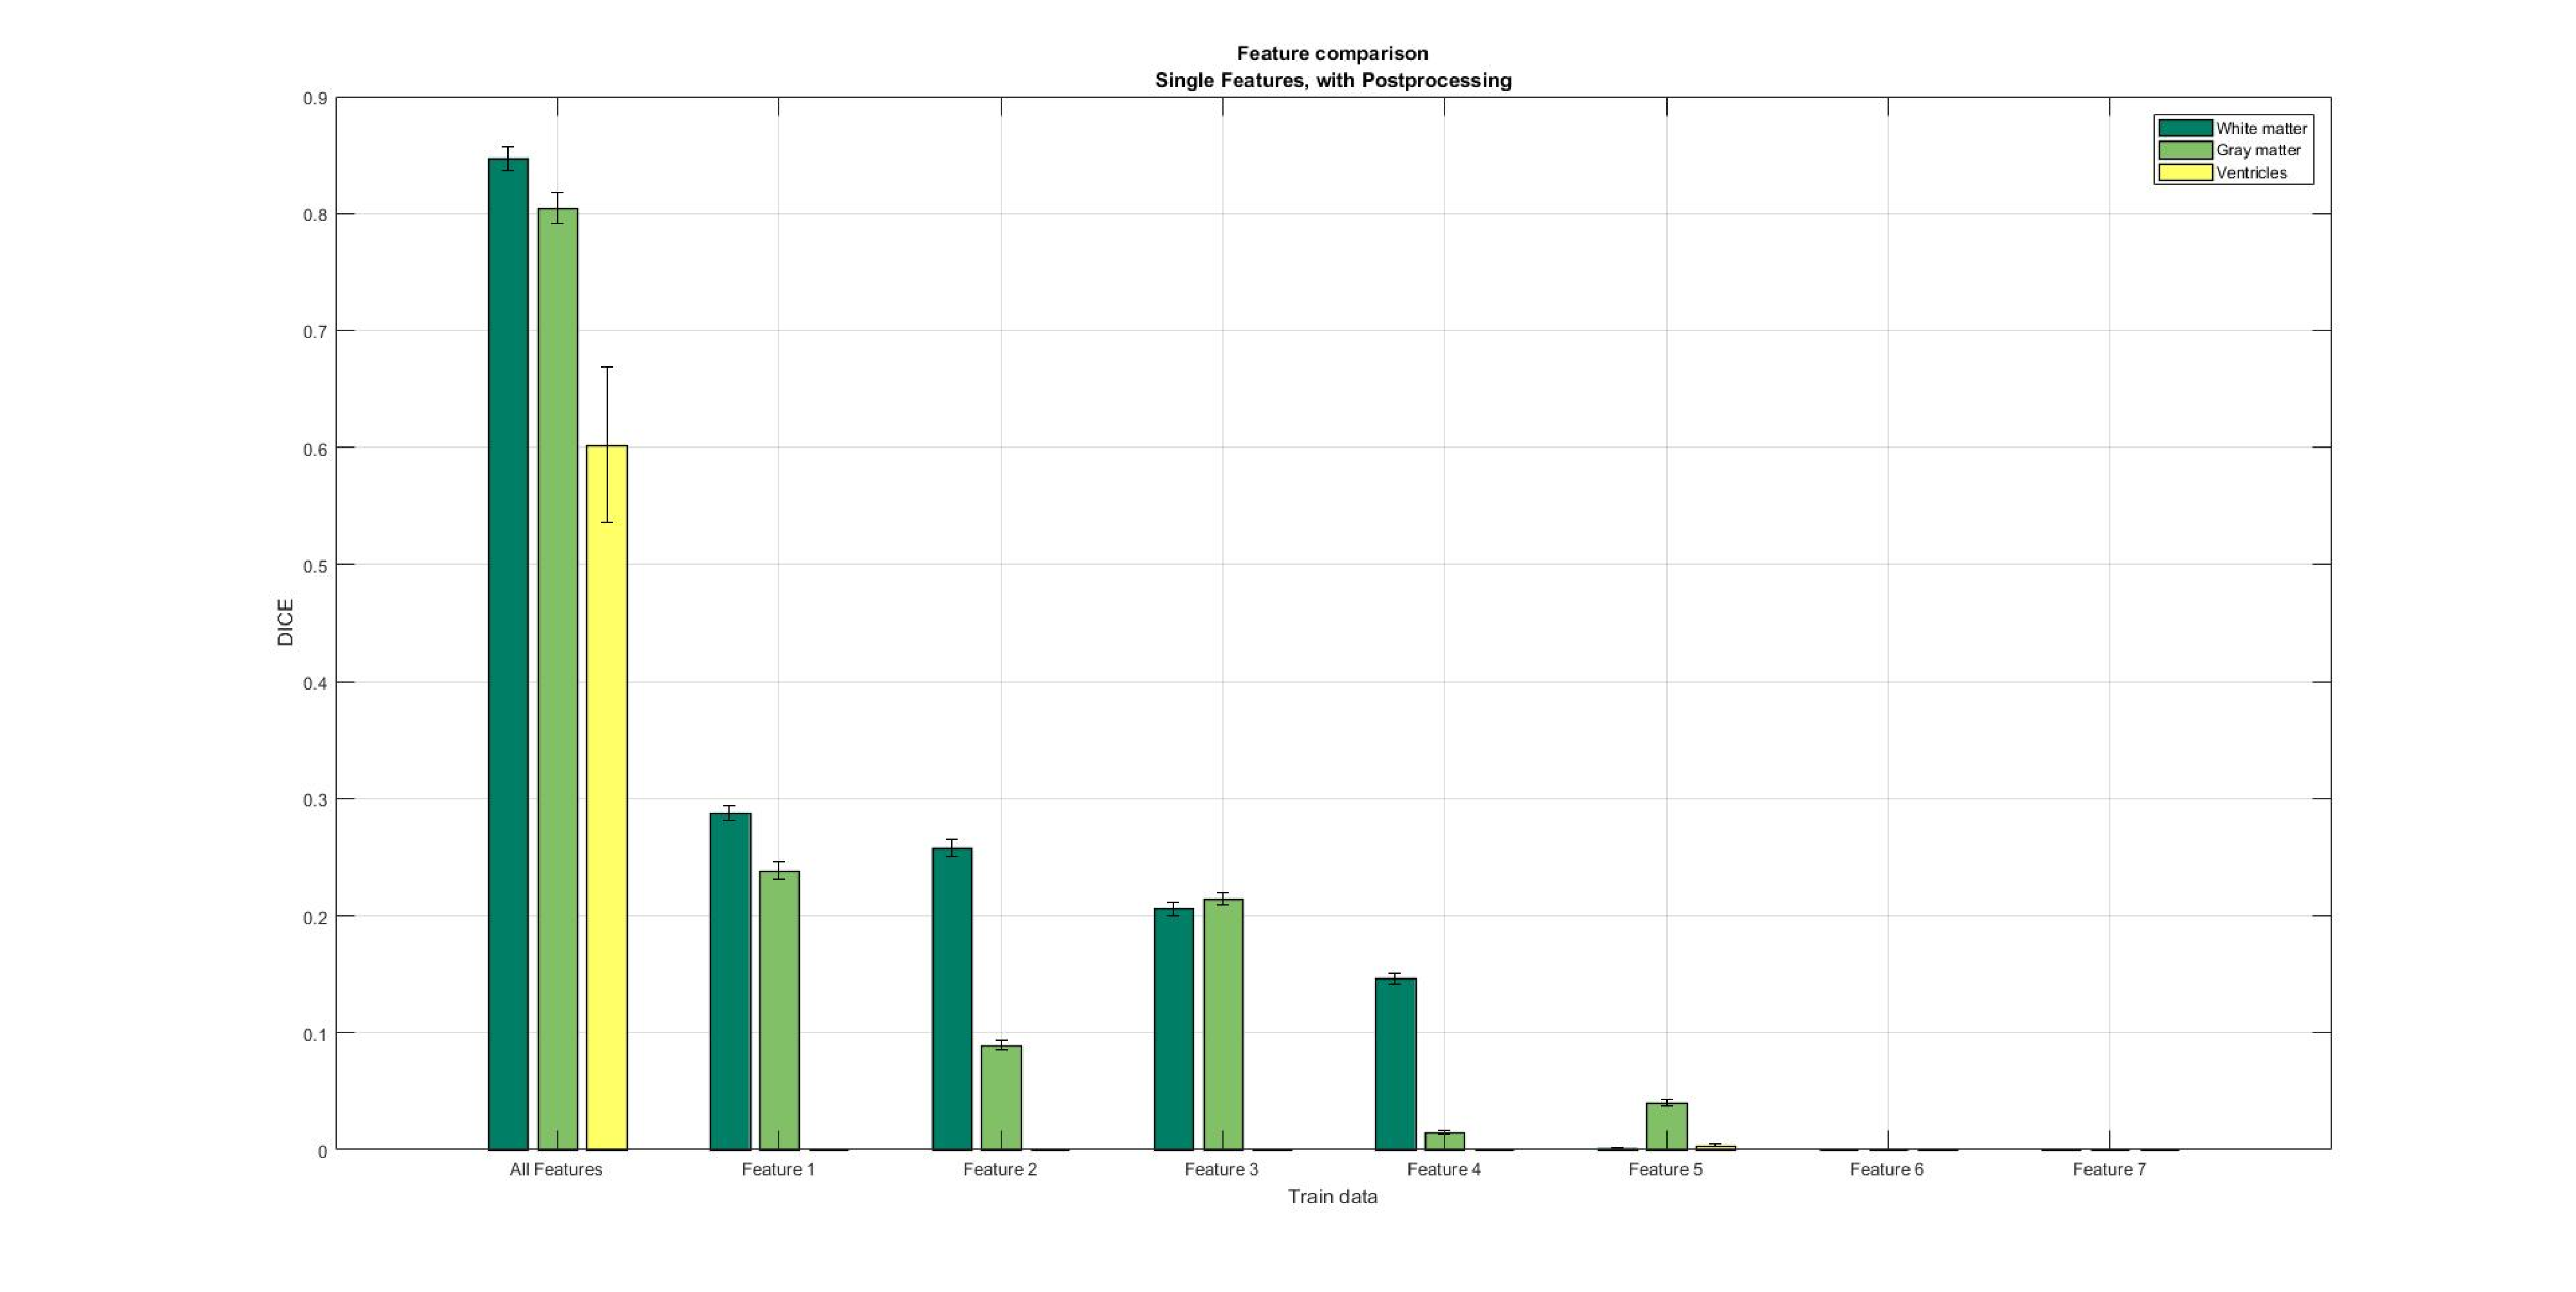
\includegraphics[width=0.48\textwidth]{images/DF_FE_SF_PP}
	\caption{Feature evaluation with Decision Forest by using a single feature and with preprocessing }
	\label{DF_FeatEval_SF_PP}
\end{figure}



\subsection{Random Mask Optimization}

One major task to handle was the low value for the ventricles. Dice values above 0.5 were hard to achieve. One way to improve the dice for ventricles was to optimize the random mask with respect to the fraction of ventricle voxels taken into account. The effects of the random mask on the ventricle dice can be seen in Fig.~(\ref{f.random_mask}). Best results were achieved with a fraction of 0.004 ventricles, approximately the same fraction as for white matter and grey matter. All following results are based on this optimized mask.
\begin{figure}[h!]
	\centering
	\subfloat[]{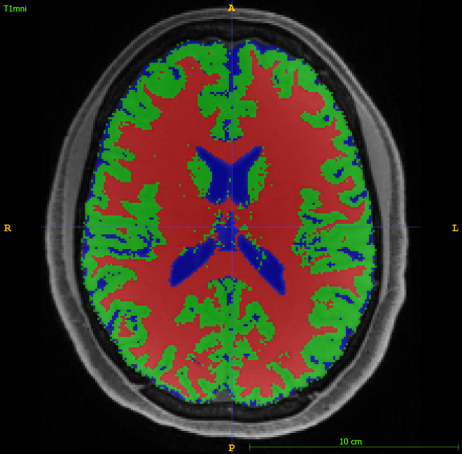
\includegraphics[width=0.3\linewidth]{images/ven_0_4}}
	\hfill
	\subfloat[]{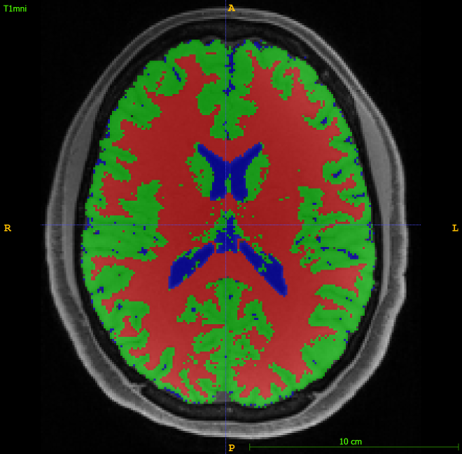
\includegraphics[width=0.3\linewidth]{images/ven_0_04}}
	\hfill
	\subfloat[]{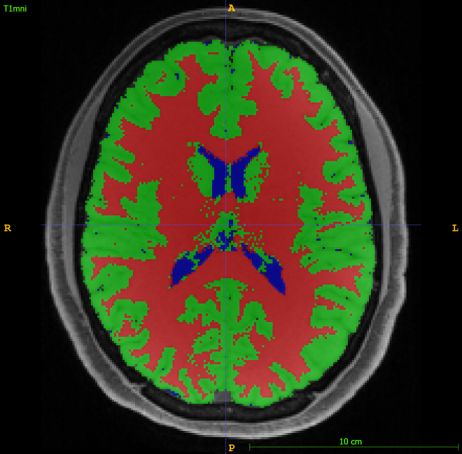
\includegraphics[width=0.3\linewidth]{images/ven_0_004}}
	\caption{Optimization of the random mask parameter for ventricles. Fraction of ventricle voxels taken into account $f_v$ and dice value for this certain parameter $d_v$ are: ($f_v$ / $d_v$) (a) 0.4 / 0.22, (b) 0.04 / 0.44, and (c) 0.004 / 0.62.}
	\label{f.random_mask}
\end{figure}


\subsection{Algorithm Performance}



The decision forest algorithm was enhanced with normalized features, a higher number of ventricle voxels in the training set and the optimization of the hyperparameters (see Fig.~\ref{f.df_white}). With this settings, the max dice coefficient was lifted from 0.703 to 0.754. This result was achieved with 80 trees and 3000 max nodes.

\begin{figure}[h!]\label{f.df_white}
	\centering
	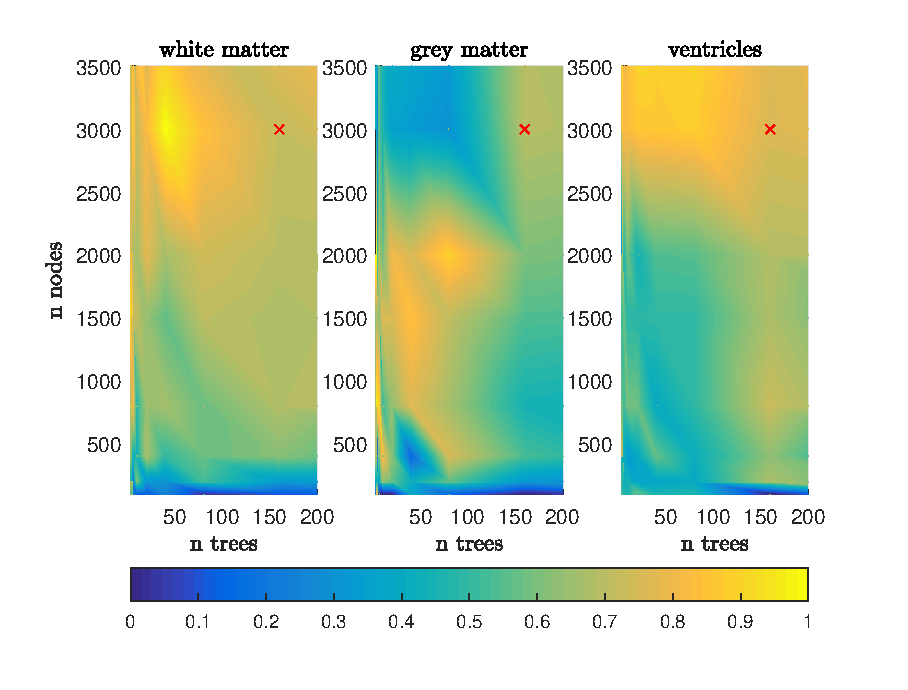
\includegraphics[width=0.48\textwidth]{images/df_grid}
	\caption{DF plot of grid search for white matter, grey matter and ventricles. The red cross marks the chosen hyperparameters number of trees~=~160 and maximum nodes per tree~=~3000. Color does not represent dice, the data is stretched individually for all three plots.}
\end{figure}



Statistical distribution of the dice coefficients can be seen in Fig. \ref{f.boxplot}. DF and SVM achieve a similar mean dice score but SVM has a lower variance for the ventricles.
\begin{figure}\label{f.boxplot}
	\centering
	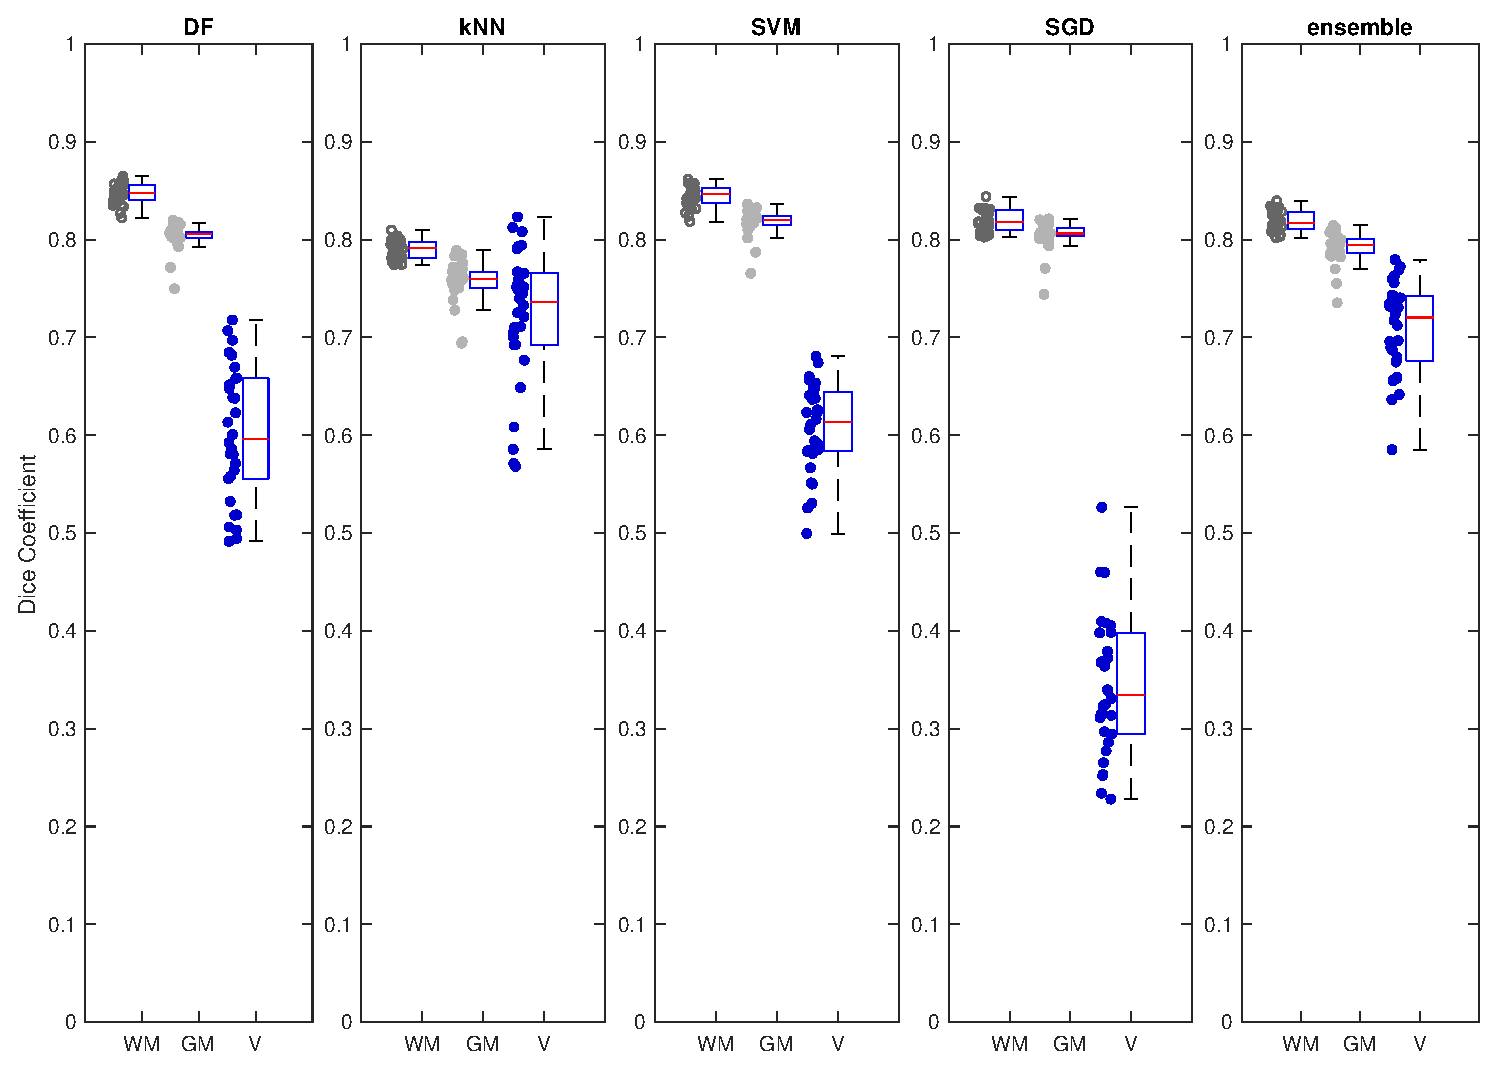
\includegraphics[width=0.48\textwidth]{images/boxplot}
	\caption{Distribution of dice coefficients with optimal hyper-parameters for each algorithm on the full training set of 70 images.}
\end{figure}

Comparison of computation time for training and testing is shown in Fig. \ref{f.runtimebarplot}.
\begin{figure}\label{f.runtimebarplot}
	\centering
	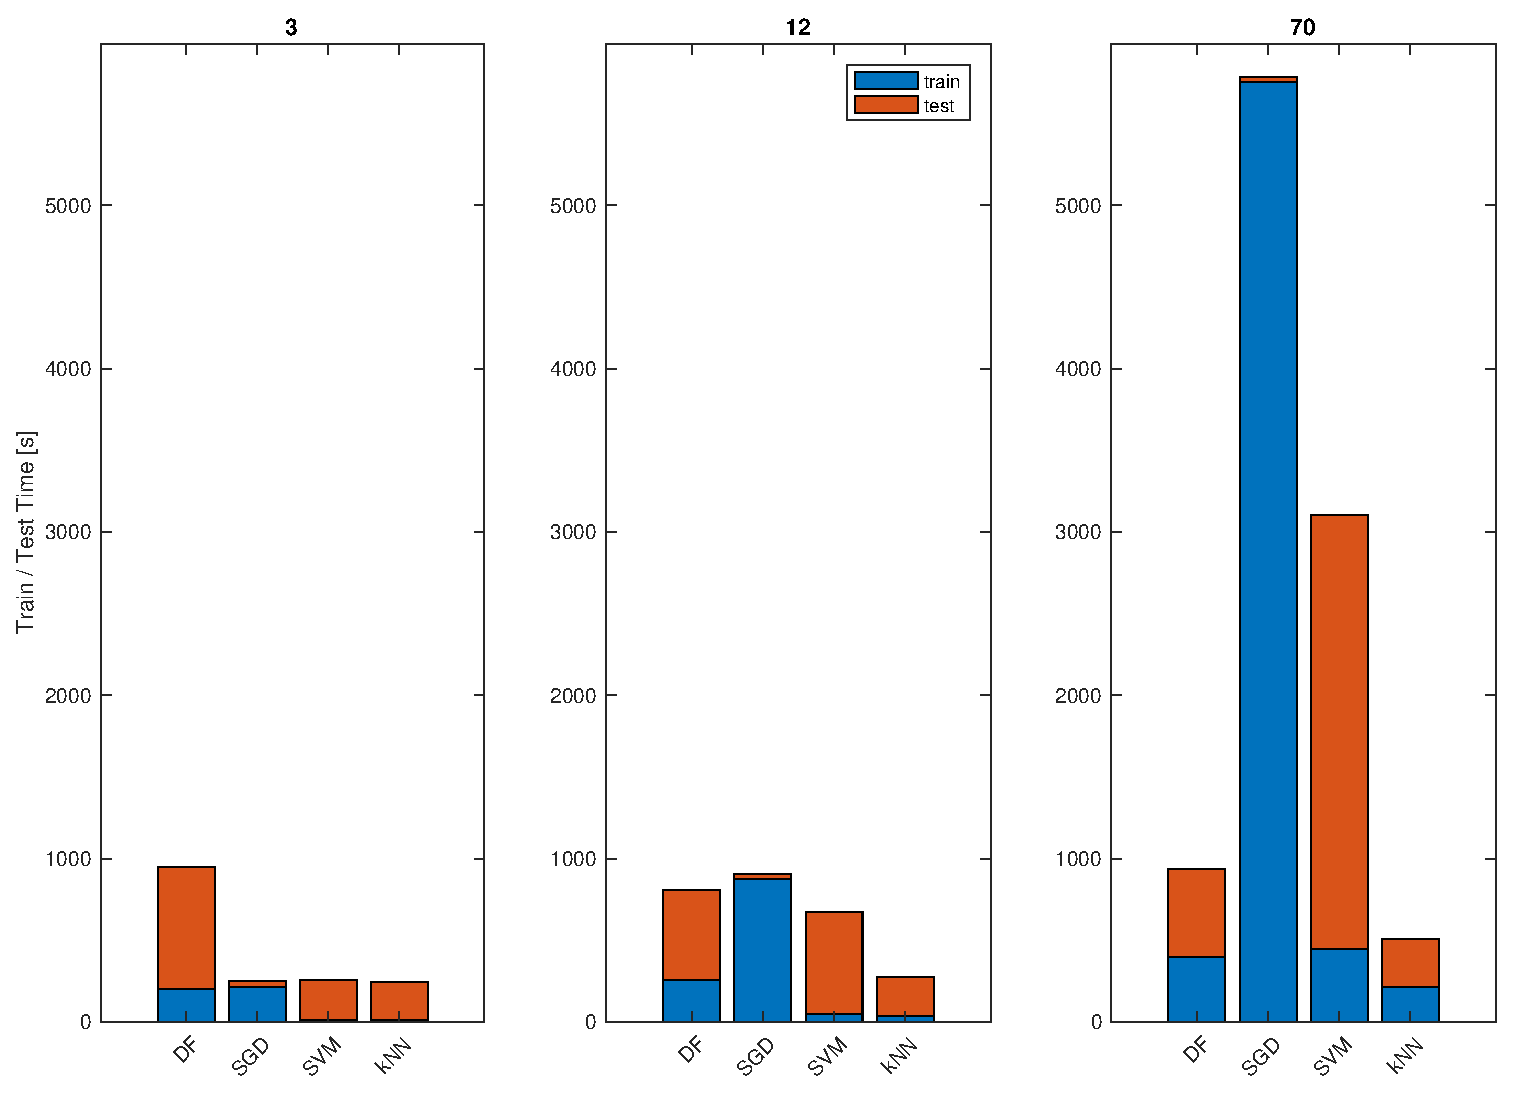
\includegraphics[width=0.48\textwidth]{images/runtimes}
	\caption{Time for training and testing of the algorithms with training set sizes of 3, 12 and 70 samples. Test time is for one sample.}
\end{figure}


\begin{table*}[t]
\renewcommand{\arraystretch}{1.2}
\newcommand\mulrow[2]{\multirow{#1}{*}{\shortstack[c]{#2}}}
\caption{Performance Comparison of ML Algorithms}
\label{tab:perf_compare}
\centering
\begin{threeparttable}
\begin{tabular*}{0.9\textwidth}{@{\extracolsep{\fill}}c*{7}{S[table-number-alignment=center,table-figures-decimal=2,table-auto-round]}@{}}
\toprule
Features & {Size Dataset} & {\shortstack[c]{DF}} & {\shortstack[c]{GMM}} & {\shortstack[c]{kNN}} & {\shortstack[c]{SGD}} & {\shortstack[c]{SVM}} & {\shortstack[c]{ensemble}}\\
\midrule
\mulrow{3}{All\\(f1-f7)}
	& 3		&	{0.85/0.81/0.62}	& {-}	& {0.70/0.57/0.50}	& {0.82/0.80/0.35}	& {0.83/0.80/0.61}	& {-}\\
	& 12	&	{0.85/0.81/0.59}	& {-}	& {0.75/0.66/0.67}	& {0.82/0.80/0.34}	& {0.84/0.81/0.61}	& {-}\\
	& 70	&	{0.85/0.80/0.60}	& {-}	& {0.80/0.76/0.72}	& {0.82/0.80/0.34}	& {0.84/0.82/0.61}	& {0.82/0.79/0.71}\\
\midrule
\mulrow{3}{Coordinates only\\(f1-f3)}
	& 3		&	{0.67/0.63/0.22}	& {-}	& {0.70/0.55/0.41}	& {0.17/0.23/0.00}	& {0.59/0.52/0.0}	& {-}\\
	& 12	&	{0.67/0.64/0.11}	& {-}	& {0.74/0.63/0.56}	& {0.19/0.22/0.00}	& {0.59/0.57/0.0}	& {-}\\
	& 70	&	{0.67/0.64/0.16}	& {-}	& {0.77/0.71/0.62}	& {0.17/0.21/0.00}	& {0.60/0.58/0.31}	& {-}\\
\midrule
\mulrow{3}{All non-coordinates \\(f4-f7)}
	& 3		&	{0.84/0.80/0.50}	& {-}	& {0.85/0.80/0.45}	& {0.82/0.80/0.34}	& {0.84/0.79/0.0}	& {-}\\
	& 12	&	{0.85/0.80/0.49}	& {-}	& {0.85/0.81/0.45}	& {0.82/0.80/0.33}	& {0.85/0.80/0.45}	& {-}\\
	& 70	&	{0.85/0.80/0.48}	& {-}	& {0.85/0.81/0.54}	& {0.82/0.80/0.34}	& {0.85/0.80/0.44}	& {-}\\
\bottomrule
\end{tabular*}
\begin{tablenotes}
\item Overview of achieved accuracy for the different algorithms. Mean dice scores for white matter/grey matter/ventricles.
\item f1-f3: Coordinate features, f4: T1 intensity, f5: T1 gradient, f6: T2 intensity, f7: T2 gradient.
\end{tablenotes}
\end{threeparttable}
\end{table*}

\begin{table*}[t]
\renewcommand{\arraystretch}{1.2}
\newcommand\mulrow[2]{\multirow{#1}{*}{\shortstack[c]{#2}}}
\caption{Runtime}
\label{tab:time_compare}
\centering
\begin{threeparttable}
\begin{tabular*}{0.9\textwidth}{@{\extracolsep{\fill}}c*{6}{S[table-number-alignment=center,table-figures-decimal=2,table-auto-round]}@{}}
\toprule
Features & {Size Dataset} & {\shortstack[c]{DF}} & {\shortstack[c]{GMM}} & {\shortstack[c]{kNN}} & {\shortstack[c]{SGD}} & {\shortstack[c]{SVM}}\\
\midrule
\mulrow{3}{All\\(f1-f7)}
	& 3		&	{205.4/22310.2}		& {-}	& {13.4/7023.7}	& {214.9/1219.6}	& {15.1/7289.7}\\
	& 12		&	{258.7/16563.6}		& {-}	& {38.1/7090.0}	& {259.9/1250.0}	& {48.2/18730.5}\\
	& 70		&	{401.4/16116.2}		& {-}	& {215.5/8873.5}	& {445.3/1279.6}	& {448.1/79668.4}\\
\midrule
\mulrow{3}{Coordinates only\\(f1-f3)}
	& 3		&	{-}		& {-}	& {10.4/4391.5}	 	& {-}	& {15.4/12178.7}\\
	& 12	&	{-}		& {-}	& {34.7/5449.3}		& {-}	& {62.2/43404.3}\\
	& 70	&	{-}		& {-}	& {196.4/6112.8}	& {-}	& {957.9/221440.5}\\
\midrule
\mulrow{3}{All non-coordinates \\(f4-f7)}
	& 3		&	{-}		& {-}	& {10.1/10084.7}	& {-}	& {12.4/6647.9}\\
	& 12	&	{-}		& {-}	& {34.6/18768.6}	& {-}	& {39.8/18691.1}\\
	& 70	&	{-}		& {-}	& {194.2/16555.7}	& {-}	& {323.2/80532.7}\\
\bottomrule
\end{tabular*}
\begin{tablenotes}
\item \FIXME{Overview of the computation time in seconds for all algorithms (training time/testing time). Computation time includes pre- and post-processing.}
\end{tablenotes}
\end{threeparttable}
\end{table*}


\section{Discussion}
\TODO{feature importance? which algorithm to choose for which use-case?}

We have observed a rather small influence of the size of the training set, DF, SGD, and SVM reaching a similar dice coefficient with either 3 or 70 training samples.


\section{Conclusion}
The major challenge in the current setup remains the quality of ground-truth data. As long as the test set is the output from an other (imperfect) algorithm, any approach is just an approximation of the other mechanism.

\section*{Acknowledgement}
Calculations were performed on UBELIX (http://www.id.unibe.ch/hpc), the HPC cluster at the University of Bern.

\bibliographystyle{IEEEtran}
\bibliography{references}

\end{document}